% Created 2024-09-03 Tue 23:37
% Intended LaTeX compiler: pdflatex
\documentclass[12pt]{article}
\usepackage[utf8]{inputenc}
\usepackage[T1]{fontenc}
\usepackage{graphicx}
\usepackage{longtable}
\usepackage{wrapfig}
\usepackage{rotating}
\usepackage[normalem]{ulem}
\usepackage{amsmath}
\usepackage{amssymb}
\usepackage{capt-of}
\usepackage{hyperref}
\usepackage[margin=1in]{geometry} \usepackage{amsmath}
\author{Jason Press}
\date{\today}
\title{Dropping Balls Onto the Floor}
\hypersetup{
 pdfauthor={Jason Press},
 pdftitle={Dropping Balls Onto the Floor},
 pdfkeywords={},
 pdfsubject={},
 pdfcreator={Emacs 29.4 (Org mode 9.8)}, 
 pdflang={English}}
\begin{document}

\maketitle
\begin{abstract}


In this lab, we obtained an experimental value of the acceleration of an object due to the gravitational force of the Earth by dropping balls. We performed two experiments: one with a Drop Box in a lab, and another dropping tennis balls off a balcony. By measuring the height and time of the drop, the we calculated the acceleration on the ball due to gravity. We obtained a value of \(g\) that contains the true value of \(g\) within the error propagation in both experiments:  \(8.3\pm2.3 \frac{\text{m}}{\text{s}^{2}}\) for the Drop Box experiment; and \(10.4\pm 0.728 \frac{\text{m}}{\text{s}^{2}}\) for the balcony experiment.
\end{abstract}
\section{Introduction}
\label{sec:org09312ae}

The aim of this lab is to measure the acceleration of an object in free fall due to the gravitational force of Earth. In order to measure the acceleration due to gravity, we performed two tests: dropping a metal ball from a Drop Box and timing and measuring the distance it fell; and dropping a tennis ball from a balcony and timing the distance it fell.

Kinematics can describe the distance an object travels with constant acceleration as a function of time with \(x\left(t\right) = x_{0} + v_{0}t + \frac{1}{2}at^{2}\), where \(x_{0}\) is the initial position, \(v_{0}\) is the initial velocity, and \(a\) is the acceleration of the object. Assuming \(x_{0}\) is the initial height of the bottom of the ball \(h\), the end position of the ball is zero, \(v_{0}\) is zero since the ball starts at rest, and \(a\) is the negative acceleration of the ball due to gravity since objects fall down, then the kinematics equation can be rearranged to describe the acceleration due to gravity:

\begin{enumerate}
\item \(x(t) = x_{0} + v_{0}t + \frac{1}{2}at^{2} \)
\item \( \text{Assume } x_{0} = h \text{, } x(t) = 0 \text{, } v_{0} = 0 \text{, and } a = -g \)
\item \(0 = h - \frac{1}{2} gt^{2} \)
\item \(g = \frac{2h}{t^{2}} \)
\end{enumerate}

Using this formula, the acceleration due to gravity can be calculated with a distance \(h\) and time \(t\).
\section{Methods}
\label{sec:org1a14315}

To minimize error, we performed two experiments: dropping a steel ball from a Drop Box in the lab; and dropping a tennis ball from a balcony.

For the first experiment, the steel ball from a Drop Box in the lab, we measured the height with a two meter meterstick to the bottom of the Drop Box where the ball rests, and the height of the ball was also measured. From this, the distance the ball falls can be calculated as \(\Delta x = x_{\text{Height to Drop Box}} - x_{\text{Height of ball}}\).

In order to determine the time the ball is in free fall, we recorded each drop with an iPhone camera. For this first experiment, the camera was filming at 30 frames per second. The time the ball begins falling the frame it initially moves from the Drop Box, and ends the frame it bounces on the ground and reverses direction. iOS allows the exact time of the frame within the video to be calculated, so the total time in free fall is the difference between the end and start time.

The Drop Box holds the ball in its initial position with an electromagnet. When we pressed the release switch, the electromagnet turns off, and the only force acting on the ball is gravity, which causes it to fall. See Figure \ref{fig:dropbox} for a visual depiction of the setup.

Since the environment is a controlled environment, we only performed five tests to minimize error across tests. We used the average height and time to calculate \(g\), and we used the standard error of the drops as part of the error propagation.

For the second experiment, the tennis ball dropped from the balcony, we measured the distance from the point of impact to the height of the top of the balcony, where we dropped the ball from, with a roll tape measure. The ball was initially placed on the balcony before moving over the edge of the balcony, making sure to not move the ball vertically. Then, we released the ball. We recorded the point of impact at the bottom, and we placed the bottom of the roll tape at the point of impact, and the other end of the roll tape at the point of drop. The measurement obtained with this was the true height the ball fell.

Similarly, for the second experiment, an iPhone camera filmed the whole drop, and we obtained the time in free fall in the same fashion as the first experiment. Unlike the first experiment, this iPhone filmed at 60 frames per second. See Figure \ref{fig:balcony} for a visual depiction of the setup.

Since the outdoors are less controlled, we performed ten trials instead of five. This allows the inherit randomness of drop to drop variations, such as a gust of wind pushing the ball, to cancel out as much as possible in the average over the ten tests. We account for the drop to drop variations in the error propagation calculations.

\begin{center}
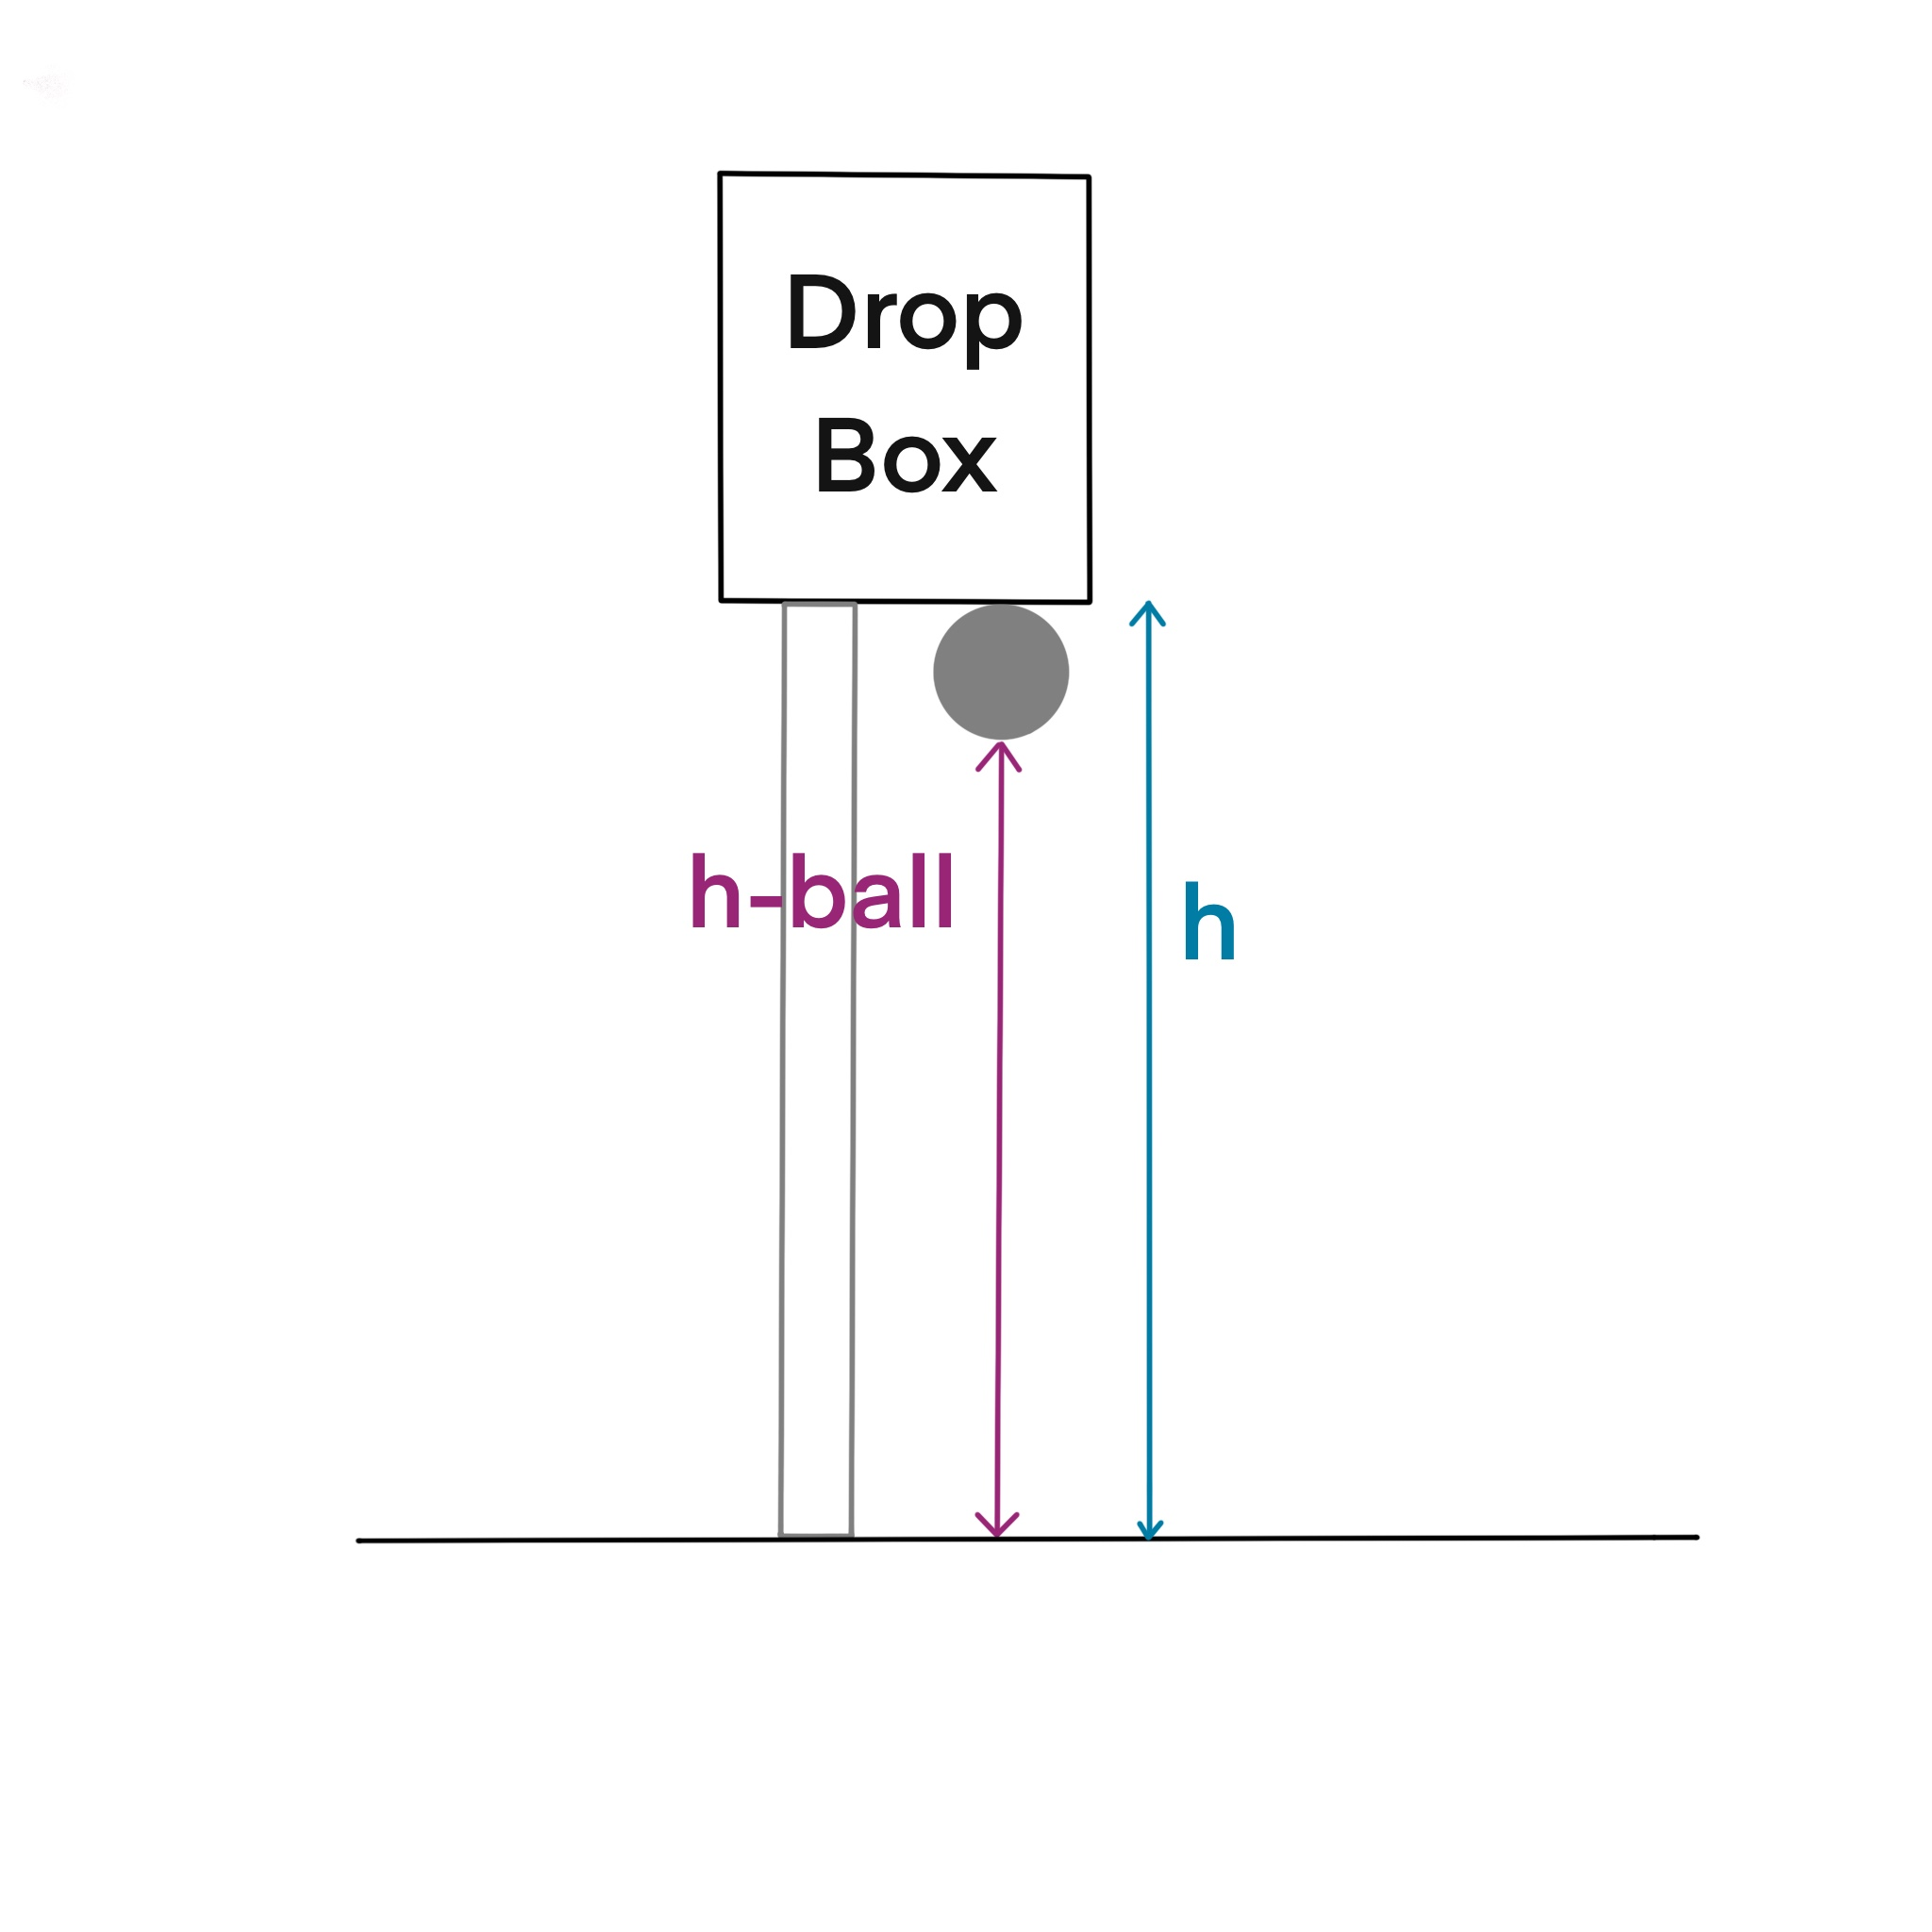
\includegraphics[height=6cm]{./dropbox.jpg}
\captionof{figure}{\label{fig:dropbox}Drop Box setup}
\end{center}

\begin{center}
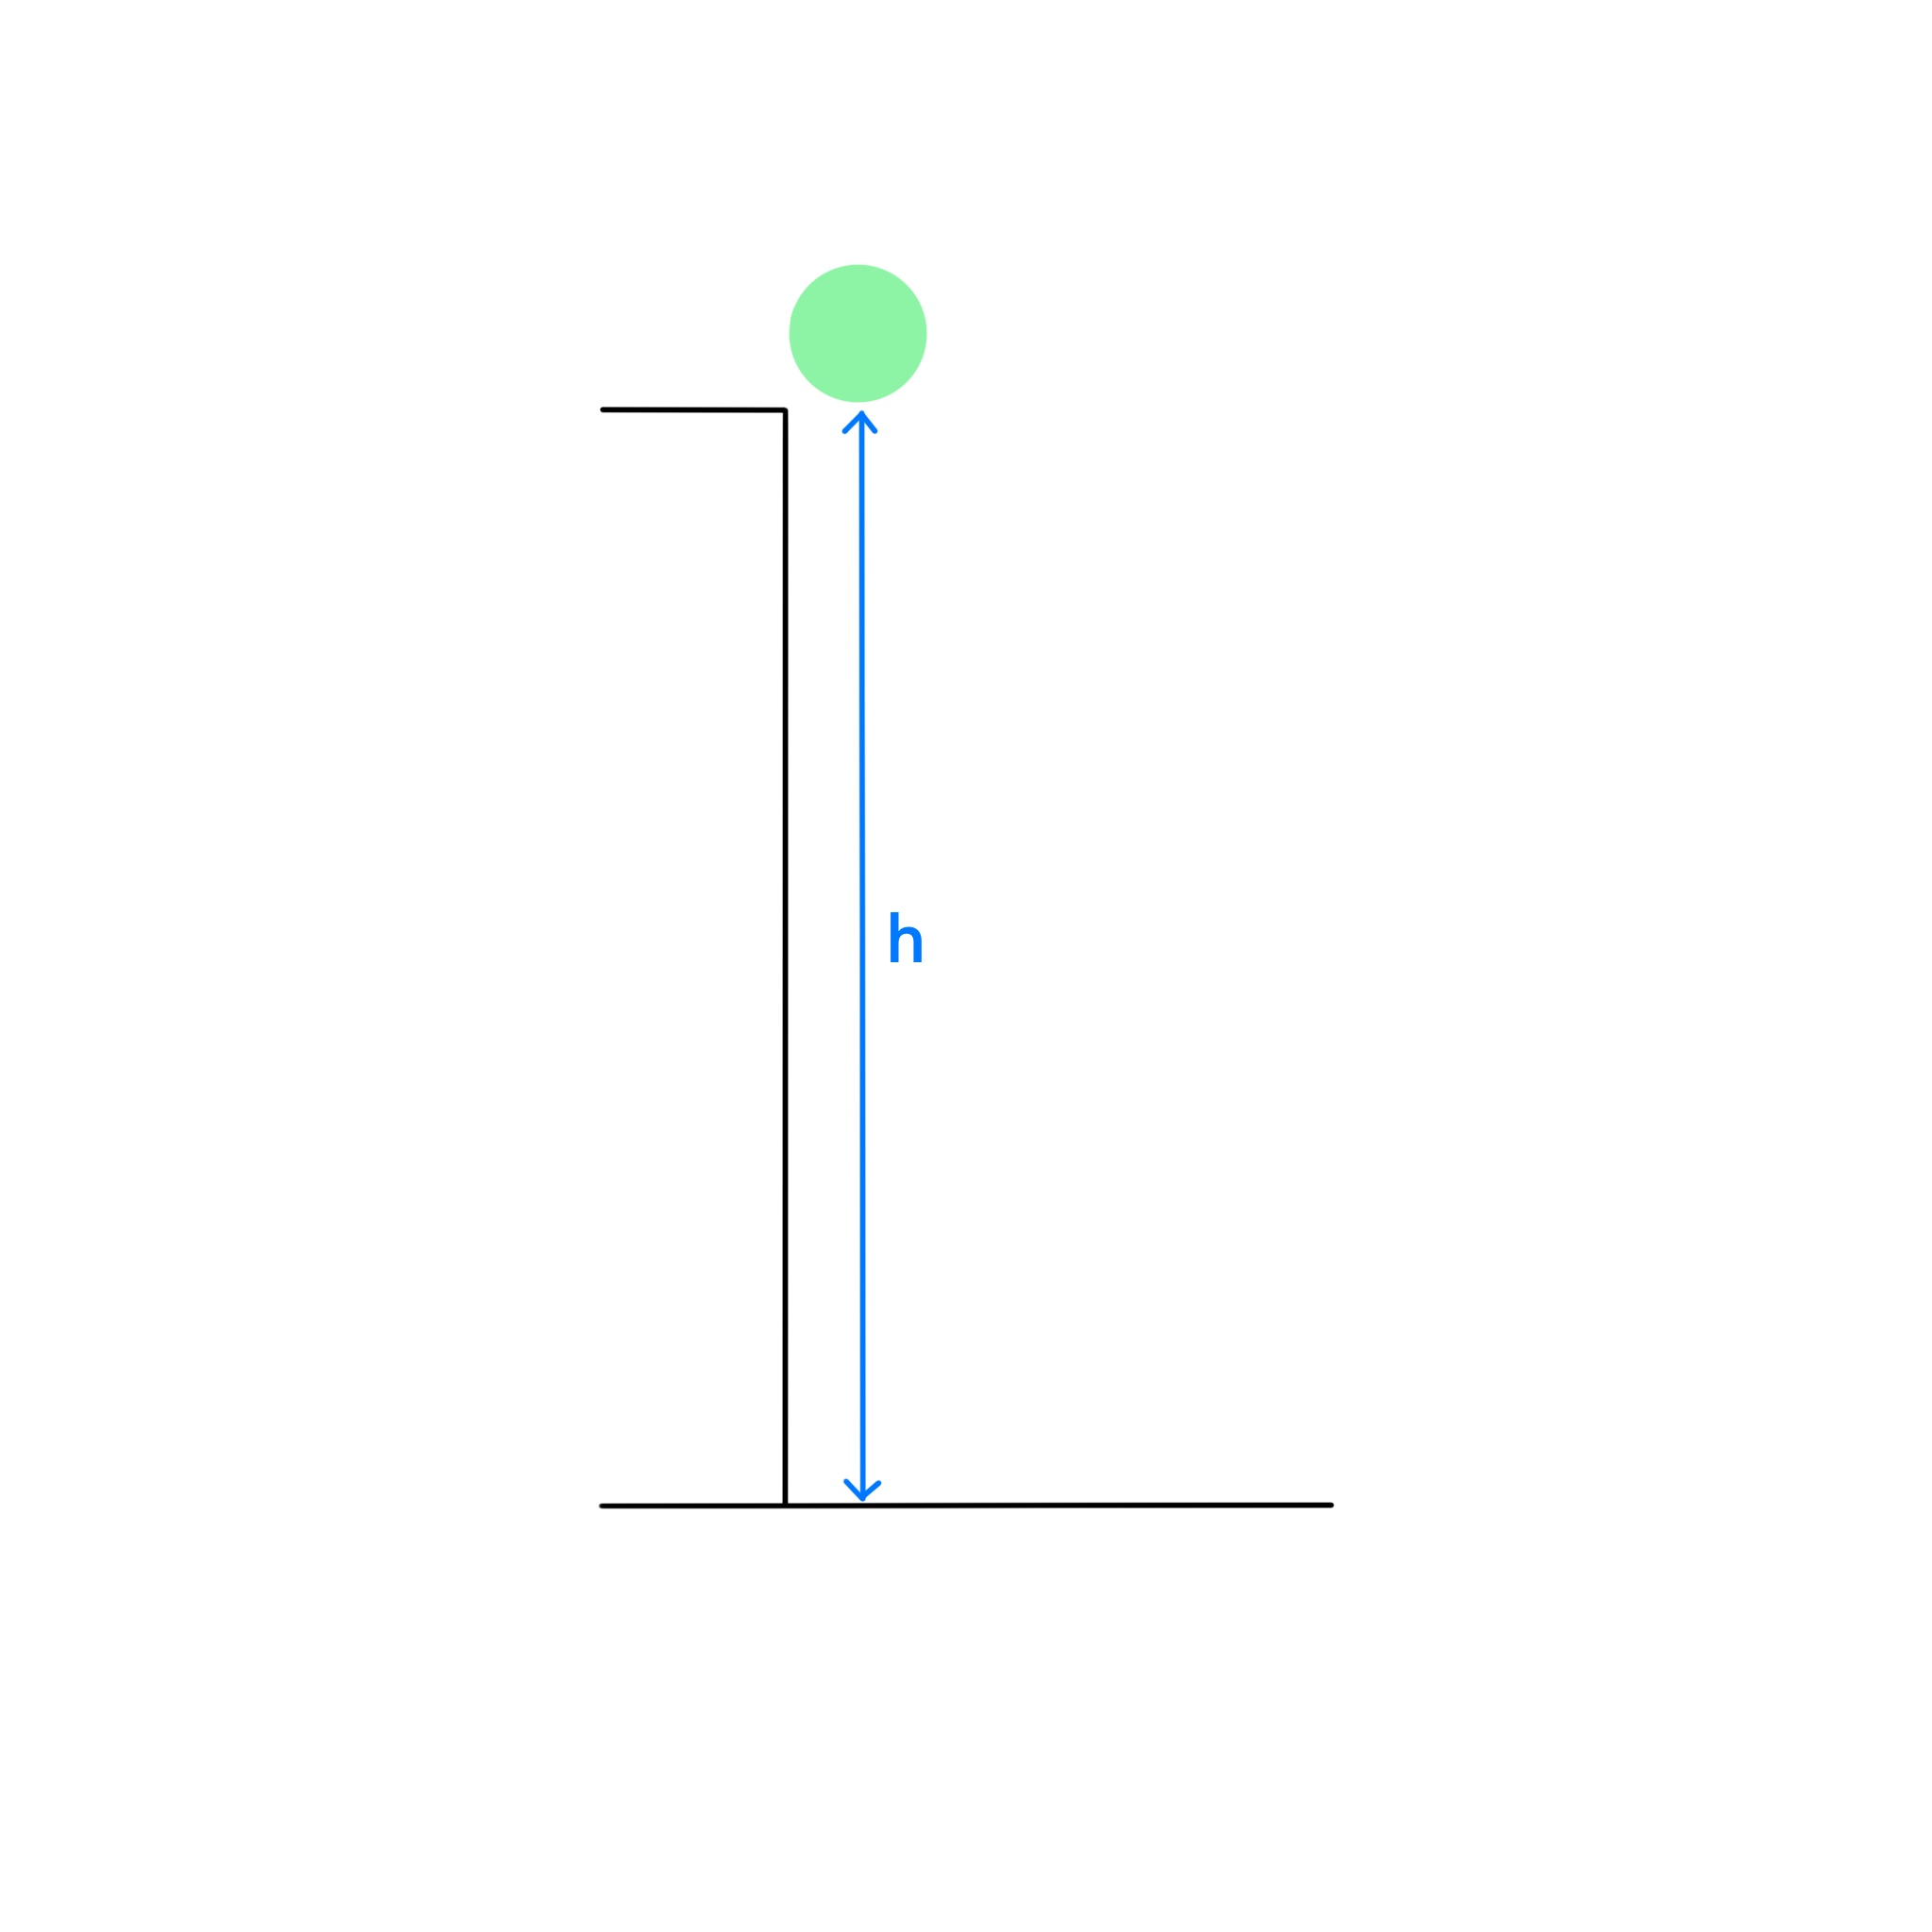
\includegraphics[height=6cm]{./balcony.jpg}
\captionof{figure}{\label{fig:balcony}Balcony drop setup}
\end{center}

Note: the figures are \emph{not} to scale.
\section{Results}
\label{sec:orgfd4685d}

\subsection{Drop Box}
\label{sec:org5d21adf}

These are the results from the Drop Box experiment.

\begin{center}
\captionof{table}{\label{table:dropbox}Drop Box results}
\begin{tabular}{r|r|r}
\hline
Run & Height (cm) & Time (s)\\
\hline
1 & 105.9 & 0.51\\
2 & 105.9 & 0.51\\
3 & 105.9 & 0.51\\
4 & 105.9 & 0.53\\
5 & 105.9 & 0.47\\
\hline
Average & 105.90 & 0.505\\
\end{tabular}
\end{center}

The calculated result of \(g\) using the averages is \(8.3\pm2.3 \frac{\text{m}}{\text{s}^{2}}\).
\subsection{Balcony}
\label{sec:orgbbf327e}

These are the results from the balcony experiment.

\begin{center}
\captionof{table}{\label{table:balcony}Balcony drop results}
\begin{tabular}{r|r|r}
\hline
Run & Height (cm) & Time (s)\\
\hline
1 & 560.0 & 1.01\\
2 & 560.0 & 1.05\\
3 & 560.0 & 1.01\\
4 & 560.0 & 1.07\\
5 & 560.0 & 1.00\\
6 & 559.6 & 1.05\\
7 & 560.0 & 1.06\\
8 & 559.6 & 1.06\\
9 & 559.8 & 1.03\\
10 & 560.2 & 1.05\\
\hline
Average & 559.92 & 1.039\\
\end{tabular}
\end{center}

The calculated result of \(g\) using the averages is \(10.4\pm 0.728 \frac{\text{m}}{\text{s}^{2}}\).

All of the calculated results contain the true value of \(g = 9.81 \frac{\text{m}}{\text{s}^{2}}\) within the calculated error propagation.
\section{Discussion}
\label{sec:orge9f4c56}

Ultimately, the purpose of this lab was to calculate the value of \(g\). The experimental value of \(g\) contained the true value of \(g\) in both experiments; \(g = 9.81 \frac{\text{m}}{\text{s}^{2}} \in 8.3\pm2.3 \frac{\text{m}}{\text{s}^{2}}\) and \(g = 9.81 \frac{\text{m}}{\text{s}^{2}} \in 10.4\pm 0.728 \frac{\text{m}}{\text{s}^{2}}\). However, there is a good amount of error.
\subsection{Calculating error}
\label{sec:org6463e07}

We calculated error using the standard formula for error propagation \(\sigma\): \(\sigma = \sqrt{\sum_{L} \frac{\partial g}{\partial L}^{2}\sigma_{L}^{2}}\) for all measurements \(L\), and \(\sigma_{L}=\sqrt{\sigma_{sys,L}^{2}+\sigma_{res,L}^{2}+\sigma_{stat,L}^{2}}\). Since there are two measurements, height and time, the formula for error propagation is \(\sigma = \sqrt{ \left( \frac{2}{t^{2}} \right) ^{2} \sigma_{h}^{2} + \left( \frac{-4h}{t^{3}} \right)^{2}\sigma_{t}^{2} }\).

The error within a measurement has three components: resolution, systematic, and statistical.

Resolution error is simply half of the resolution of the measuring device. The roll tape has a resolution of 0.2cm, so the resolution error is 0.1cm. For a 30 frames per second video, the resolution is half of the length of a frame, or \(\frac{1}{60}\)s.

Systematic error is the amount of variability between measurements. For the distance measurements, our group used the resolution error, since we were confident in our measurements of distance. Additional repeated measurements of the same known objects yielded values within the resolution error. For the video measurements, we gave one frame of error for the drop, since noticing the beginning of the ball's movement is tricky, and one frame of error for the time it took to hit the ground, since the ball headed down in one frame and up in the other: the actual bounce was never recorded. This gives two frames of error. For a 30 frames per second video, the systematic error is 2 frames, or \(\frac{2}{30}\)s.

Statistical error is the amount of variability by external factors, such as wind. To account for this variability, we use the estimate for standard error \(\sigma_{sys} = \frac{\sigma}{\sqrt{n}}\), where \(\sigma\) is the standard deviation of the measurements and \(n\) is the number of measurements.

For the Drop Box experiment, we only used five drops to minimize the run to run variability since the lab is a controlled environment. However, for the balcony experiment, we used ten drops since there were more sources of systematic error, such as wind, not holding the ball at the perfect height (i.e. moving the ball slightly up or down while bringing it into the dropping position from the balcony ledge).
\subsection{Drop Box error}
\label{sec:orgbb7864e}

This result is surprising. Our group expected this to have the smallest error of the two experiments since it was the most controlled of the two experiments, but instead it had the largest error of the two experiments. Here is the calculated error propagation:

\begin{table}[htbp]
\caption{\label{dropbox-error}Error propagation for the Drop Box experiment}
\centering
\begin{tabular}{l|l}
\hline
\(\sigma_h\) & 0.000707m\\
\(\sigma_{h,sys}\) & 0.0005m\\
\(\sigma_{h,stat}\) & 0m\\
\(\sigma_{h,res}\) & 0.0005m\\
\hline
\(\sigma_t\) & 0.0694s\\
\(\sigma_{t,sys}\) & 0.0667s\\
\(\sigma_{t,stat}\) & 0.00980s\\
\(\sigma_{t,res}\) & 0.0167s\\
\hline
\(\frac{\partial g}{\partial h}\) & 7.842s\textsuperscript{-2}\\
\(\frac{\partial g}{\partial t}\) & -32.89\(\frac{\text{m}}{\text{s}^{3}}\)\\
\hline
\(\left(\frac{\partial g}{\partial h}\right)^{2}\sigma_{h}^2\) & 0.00003075\(\frac{\text{m}^{2}}{\text{s}^{4}}\)\\
\(\left(\frac{\partial g}{\partial t}\right)^{2}\sigma_{t}^2\) & 5.213 \(\frac{\text{m}^{2}}{\text{s}^4}\)\\
\hline
Error & \(\pm 2.3 \frac{\text{m}}{\text{s}^{2}}\)\\
\end{tabular}
\end{table}

The cause for the large error is the large magnitude of \(\left(\frac{\partial g}{\partial t}\right)^{2}\sigma_{t}^2\), suggesting a majority of the error arose in the measurement of time. For future labs, we will use a higher frame rate in video recordings to reduce the amount of error in video recordings: it becomes easier with more frames to identify the frame the ball begins to fall and the frame the ball impacts the ground, leading to an overall smaller \(\sigma_{t,sys}\).

Originally, this experiment used a photogate to get an exact time for the ball to drop, but the photogate was out of commission for this lab. If we used the photogate instead of the iPhone camera, \(\sigma_t\) would be smaller.
\subsection{Balcony error}
\label{sec:org77d4c8b}

The amount of error in this lab is about what our group expected. However, there are other factors that did not factor into our calculation of error prediction in this lab.

The big element of error in this lab that we did not account for is air resistance. As the tennis ball falls faster, the amount of drag on the tennis ball increases exponentially. To minimize air resistance, we used the lowest available balcony to allow the ball to fall from a consistent and reasonable height, but not high enough to the point where air resistance becomes a significant factor on the amount of time it takes for the tennis ball to hit the ground. The effect of air resistance would slow the ball down, increasing the time in free fall, which would increase the experimental value of \(g\).

For the tennis ball, this is a significant concern, since the height of the drop is large and the tennis ball is light relative to its size, especially when compared to the metal ball dropped from the Drop Box. Since the tennis ball is light relative to its size, the overall force of gravity acting on the tennis ball is small, so even a small amount of drag starts to have an effect on the acceleration and fall duration. However, even with a drop height of 5.6 meters, the tennis ball did not have enough time to get up to a significant speed where drag becomes significant enough of a force to seriously change the outcome of the experiment.

The calculated value for \(g\) is higher than the actual value of \(g\), suggesting a systematic error in the measurement: either the height is incorrectly measured too high, or the time measurement is too low. The most plausible explanation for this is that the time measurement is too low, meaning the ball was falling for more time than observed in the video. The frame where the ball hits the ground is easy to tell, since that is when the ball changes direction. However, choosing the correct frame for the ball starting its fall is difficult. There was most likely a number of frames that were not accounted for where the ball is in free fall but not moving a noticeable amount, yielding a shorter observed fall time relative to the actual fall time.
\section{Sample Calculations}
\label{sec:org8752076}

We used a spreadsheet to do our calculations. To find the average of times and distances, we did \texttt{=AVERAGE(A2:A11)} with whatever the start and stop range of the actual cells was (Note that \emph{specifically for the heights in cm} we did \texttt{=AVERAGE(A2:A11)/100} to convert from cm to m). After repeating for time, we found the experimental value of \(g\) with \texttt{=A13*2(B13)\textasciicircum{}2}.

To calculate standard deviation, we did \texttt{=STDEV(A2:A11)}. To get \(\sigma_{h,stat}\), we performed \texttt{=STDEV(A2:A11)/SQRT(COUNT(A2:A11))}. After manually entering \(\sigma_{h,res}\) and \(\sigma_{h,sys}\), we set \(\sigma_{h}\) \texttt{=SQRT(F6\textasciicircum{}2+F7\textasciicircum{}2+F8\textasciicircum{}2)}. After repeating similar steps for \(\sigma_t\), we obtained the error propagation with \texttt{=SQRT((2/(B13)\textasciicircum{}2)\textasciicircum{}2*F6\textasciicircum{}2+(-4*(A13)/(B13)\textasciicircum{}3)\textasciicircum{}2*I5\textasciicircum{}2)}.

The reason there are more intermediate steps for the Drop Box spreadsheet is to obtain the numbers used in Table \ref{dropbox-error}.

\begin{center}
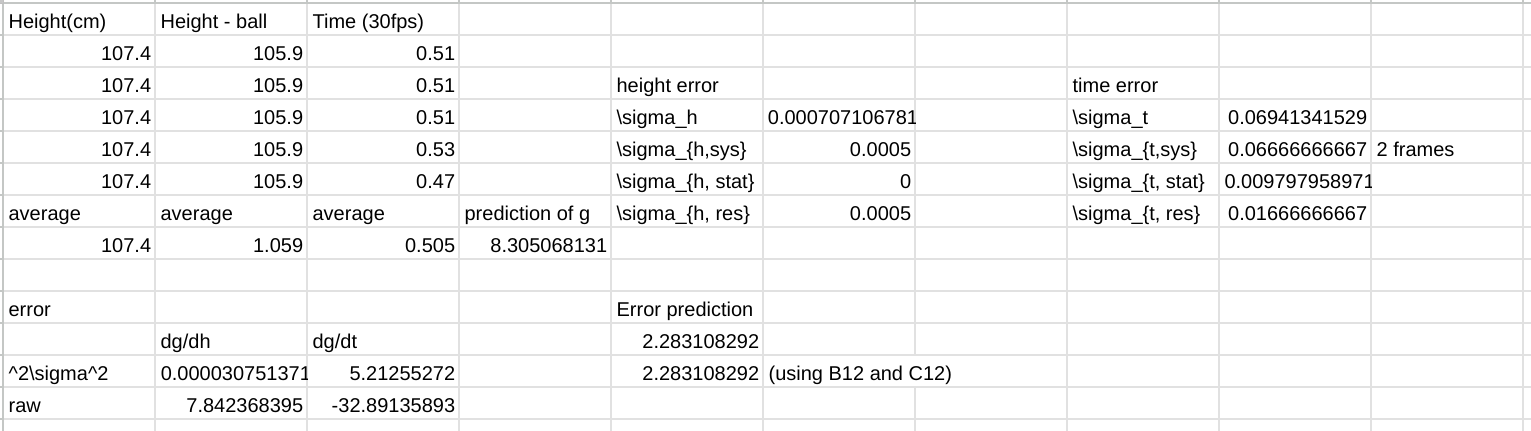
\includegraphics[width=6in]{./dropboxspreadsheet.png}
\captionof{figure}{Drop Box experiment spreadsheet}
\end{center}

\begin{center}
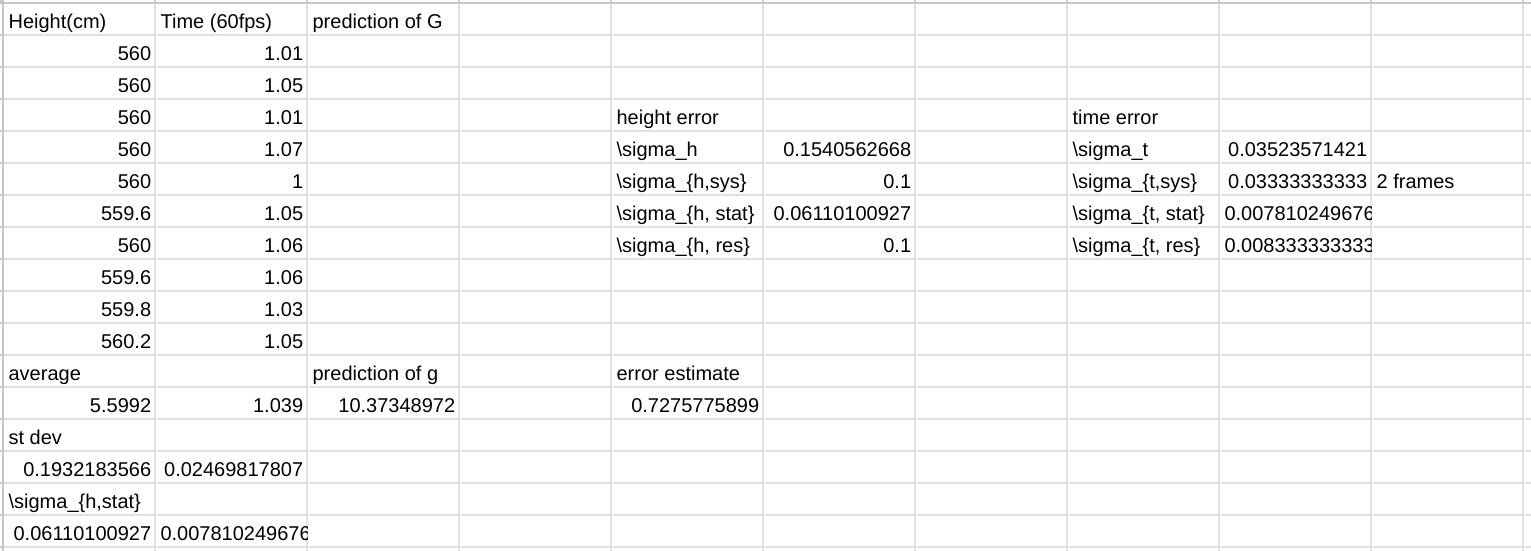
\includegraphics[width=6in]{./tennisballspreadsheet.png}
\captionof{figure}{Balcony experiment spreadsheet}
\end{center}
\end{document}
